%%%%%% NOTES %%%%%%%
% Uncomment for layout with notes
%\documentclass[handout]{beamer}
%\usepackage{pgfpages}
%\pgfpagesuselayout{4 on 1}[a4paper,border shrink=5mm]

\documentclass[table, svgnames,dvipsnames,14pt, aspectratio=169]{beamer}

%\usepackage{multirow}
%\usepackage{array}
\usepackage{booktabs}
\usepackage{graphicx}
\usepackage{fontawesome} %% for social media icons
%\usepackage{adjustbox}
\usepackage{relsize}
\usepackage[font=footnotesize, labelformat=empty, justification=raggedright]{caption}
%\usepackage{booktabs}
\usepackage{xspace}
%\usepackage{threeparttable}
%\usepackage{pgfgantt}
\usepackage{textpos}
\usepackage{fancybox}
%\usepackage{appendixnumberbeamer}
%\setbeamertemplate{page number in head/foot}[appendixframenumber]
\usepackage[framemethod=tikz]{mdframed}
%%$\usepackage{enumitem}
%%%Font change
\usepackage[T1]{fontenc}
\usepackage{cmbright} %%maybe too comic sans-y?
%
%\usepackage[latin1]{inputenc}
%%\usepackage{color}
%%\usepackage{appendixnumberbeamer}
%%\hypersetup{colorlinks,linkcolor=,urlcolor=blue}
%%\usepackage{adjustbox}
\usepackage{animate}
%\usepackage{glossaries}
\usepackage{tikz}
\usetikzlibrary{arrows,positioning, shapes.symbols,shapes.callouts,patterns, shapes, backgrounds, arrows.meta, decorations.pathreplacing} %,shapes.emoticon}
%\usepackage[export]{adjustbox}
%
%\usepackage{hyperref}
% Preamble!! :)


%\usepackage{pgfgantt}
\setbeamercovered{dynamic}


%\usepackage{appendixnumberbeamer} % use this for extra slides (appendix)

%\usetheme{bjeldbak}

\setbeamertemplate{note page}[plain]
% No navigation
\setbeamertemplate{frametitle}
  {\begin{centering}\smallskip
   \insertframetitle\par
   \smallskip\end{centering}}
\setbeamertemplate{itemize item}{$\bullet$}
\setbeamertemplate{navigation symbols}{}



% Colours
%\definecolor{Berry}{RGB}{194, 52, 102}
%\definecolor{Forest}{RGB}{33, 106, 18}
%\definecolor{Orange}{RGB}{222, 93, 59}
%\definecolor{DarkCharcoal}{HTML}{4D4944}
%\colorlet{DarkForest}{Forest!80!black}
%\colorlet{DarkOrange}{Orange!80!black}
%\colorlet{Charcoal}{DarkCharcoal!85!white}
%\colorlet{DarkBerry}{Berry!60!black}
% New Colours :)
%\definecolor{Navy}{RGB}{3, 1, 44}
%\definecolor{Purple}{RGB}{65, 34, 52}
%\definecolor{PrettyGreen}{RGB}{47, 86, 75}
%\definecolor{Pink}{RGB}{255, 105, 120}
%\definecolor{OffWhite}{RGB}{255, 234, 208}
%\colorlet{WhiteOffWhite}{OffWhite!95!white}
%\definecolor{GreyWhite}{RGB}{255,234,208}
%\definecolor{DarkPurple}{RGB}{51, 41, 56}
%\definecolor{LightishPurple}{RGB}{109, 64, 87}
\definecolor{Pinky}{RGB}{229, 104, 97}
%\definecolor{Robin}{RGB}{172, 229, 223}
%\colorlet{DarkRobin}{Robin!80!black}
%\colorlet{LightNavy}{Navy!50!white}

% New color scheme maybe!
\definecolor{DKoamaru}{HTML}{2B4162}
\definecolor{Peach}{HTML}{FFB4A2}
\definecolor{DSparkle}{HTML}{385F71}
\definecolor{Wine}{HTML}{381D2A}
\definecolor{PurpNav}{HTML}{4D5382}
\definecolor{Smoke}{HTML}{F5F0F6}
\definecolor{Carrot}{HTML}{F9A03F}
\definecolor{TerraCotta}{HTML}{E87461}
\definecolor{Eggplant}{HTML}{5E4352}
\definecolor{paleyellow}{HTML}{FDEF8D}
\definecolor{paleblue}{HTML}{769FAE}
\definecolor{palepurple}{HTML}{C0A9B0}
\definecolor{cadet}{HTML}{5CA4A9}
%\definecolor{orangeyellow}{HTML}{FFD166}
%\definecolor{orangeyellow}{HTML}{F39237}
\definecolor{orangeyellow}{HTML}{E9B44C}
%\definecolor{orangeyellow}{HTML}{F5853F}

%%%%%%% defence colours
\definecolor{newgreen}{HTML}{628062}
\definecolor{outerspace}{HTML}{444554}
\definecolor{pinkaccent}{HTML}{CC7E85}
\definecolor{darkfill}{HTML}{764248}
\definecolor{tealblue}{HTML}{33658A}

\definecolor{lightblue}{HTML}{AED9E0}
\definecolor{darkblue}{HTML}{506366}
\definecolor{lightpink}{HTML}{FE9992}
\definecolor{darkpink}{HTML}{A2625D}


%%%%%%% new palette


\definecolor{midnightpurp}{HTML}{631D76}
\definecolor{magentahaze}{HTML}{9E4770}
\definecolor{coralreef}{HTML}{FF7E6B}
\definecolor{lapis}{HTML}{2274A5}
\definecolor{warmblack}{HTML}{003844}



%%%%%%%%%%
% Use the colors: %
%%%%%%%%%%

%\setbeamercolor{title}{fg=DarkForest}
%\setbeamercolor{frametitle}{fg=DarkBerry}
%\setbeamercolor{normal text}{fg=DarkCharcoal}
%\setbeamercolor{block title}{fg=black,bg=Forest!25!white}
%\setbeamercolor{block body}{fg=black,bg=Forest!25!white}
%\setbeamercolor{alerted text}{fg=DarkOrange}
%\setbeamercolor{itemize item}{fg=Charcoal}
%\setbeamercolor{framesource}{fg=gray}
%\setbeamercolor{section in toc}{fg=DarkForest}
%\setbeamercolor{footnote}{fg=DarkCharcoal}
%\setbeamercolor{footnote mark}{fg=DarkCharcoal}
%\setbeamercolor{myfootlinetext}{fg=DarkCharcoal}
%\setbeamertemplate{itemize subitem}{\color{DarkForest}$\blacktriangleright$} % change sublist bullet to DarkForest


% New colours!
\setbeamercolor{title}{fg=warmblack}
\setbeamercolor{frametitle}{fg=white, bg=lapis}
\setbeamercolor{normal text}{fg=warmblack}
\setbeamercolor{block title}{fg=white,bg=magentahaze}
\setbeamercolor{block body}{fg=outerspace,bg=magentahaze!25!white}
\setbeamercolor{alerted text}{fg=magentahaze}
\setbeamerfont{alerted text}{series=\bfseries}
\setbeamercolor{itemize item}{fg=lapis}
\setbeamercolor{framesource}{fg=lapis}
\setbeamercolor{section in toc}{fg=midnightpurp}
\setbeamercolor{footnote}{fg=warmblack}
\setbeamercolor{footnote mark}{fg=warmblack}
\setbeamercolor{myfootlinetext}{fg=warmblack}
\setbeamertemplate{itemize subitem}{\color{lapis}$\blacktriangleright$}
\setbeamertemplate{itemize subsubitem}{\color{lapis}$\blacktriangleright$}
\setbeamertemplate{itemize item}[circle]
\setbeamercolor*{enumerate item}{fg=warmblack}
\setbeamercolor*{enumerate subitem}{fg=warmblack}
\setbeamercolor*{enumerate subsubitem}{fg=warmblack}
\setbeamerfont{frametitle}{size=\Large} % Larger slide title font
\setbeamertemplate{section in toc}[sections numbered] % numbered TOC sections
\setbeamertemplate{frametitle}[default][left] %centeredframe tittle
\setbeamertemplate{footline}[frame number]
\setbeamerfont{footnote}{size=\tiny} % set footnote font size smaller
\setbeamercolor{button}{bg=magentahaze,fg=white}



%\setbeamercolor{title}{fg=outerspace}
%\setbeamercolor{frametitle}{fg=white, bg=newgreen}
%\setbeamercolor{normal text}{fg=Wine}
%\setbeamercolor{block title}{fg=white,bg=lightpink}
%\setbeamercolor{block body}{fg=outerspace,bg=lightpink!25!white}
%\setbeamercolor{alerted text}{fg=lightpink}
%\setbeamerfont{alerted text}{series=\bfseries}
%\setbeamercolor{itemize item}{fg=darkfill}
%\setbeamercolor{framesource}{fg=lightpink}
%\setbeamercolor{section in toc}{fg=darkfill}
%\setbeamercolor{footnote}{fg=darkfill}
%\setbeamercolor{footnote mark}{fg=darkfill}
%\setbeamercolor{myfootlinetext}{fg=darkfill}
%\setbeamertemplate{itemize subitem}{\color{darkfill}$\blacktriangleright$}
%\setbeamertemplate{itemize subsubitem}{\color{darkfill}$\blacktriangleright$}
%\setbeamertemplate{itemize item}[circle]
%\setbeamercolor*{enumerate item}{fg=darkfill}
%\setbeamercolor*{enumerate subitem}{fg=darkfill}
%\setbeamercolor*{enumerate subsubitem}{fg=darkfill}
%\setbeamerfont{frametitle}{size=\Large} % Larger slide title font
%\setbeamertemplate{section in toc}[sections numbered] % numbered TOC sections
%\setbeamertemplate{frametitle}[default][left] %centeredframe tittle
%\setbeamertemplate{footline}[frame number]
%\setbeamerfont{footnote}{size=\tiny} % set footnote font size smaller
%\setbeamercolor{button}{bg=darkfill,fg=white}


%\setbeamertemplate{footline[textline]}{%
%\hfill\hspace{0.5cm} \scriptsize\sf\color{black!60}\insertframenumber{}/\inserttotalframenumber}

%\setbeamertemplate{footline}[text line]{%
%  \hfill\strut{%
%      \scriptsize\sf\color{black!60}%
%     \quad\insertframenumber
 %   }%
 %   \hfill
%}

% Macros
\newcommand{\bi}{\begin{itemize}}
\newcommand{\ei}{\end{itemize}}
\newcommand{\be}{\begin{enumerate}}
\newcommand{\ee}{\end{enumerate}}
%\newcommand{\esa}{\textit{E.\,salsugineum}}
\newcommand{\esa}{\textit{Eutrema}}
% source at bottom left of slide
\newcommand{\sourceleft}[1]{\begin{textblock*}{4cm}(0.3cm,8.8cm)
    \begin{beamercolorbox}[ht=0.5cm,left]{framesource}
        \usebeamerfont{framesource}\usebeamercolor[fg]{framesource}
{#1}
    \end{beamercolorbox}
\end{textblock*}}

% source at bottom right of slide
\newcommand{\sourceright}[1]{\begin{textblock*}{4cm}(8.6cm,8.8cm)
    \begin{beamercolorbox}[ht=0.5cm,left]{framesource}
        \usebeamerfont{framesource}\usebeamercolor[fg]{framesource}
{#1}
    \end{beamercolorbox}
\end{textblock*}}

\newcommand{\sourceextremeright}[1]{\begin{textblock*}{4cm}(10.6cm,8.8cm)
    \begin{beamercolorbox}[ht=0.5cm,left]{framesource}
        \usebeamerfont{framesource}\usebeamercolor[fg]{framesource}
{#1}
    \end{beamercolorbox}
\end{textblock*}}

% TOC shows at beginning of section
%\AtBeginSection[]
%{%
%   \begin{frame}
%       \frametitle{Overview}
%       \tableofcontents[currentsection,hideothersubsections]
%   \end{frame}
%}

% To continue enumerate counts on another slide
\newcounter{saveenumi}
\newcommand{\seti}{\setcounter{saveenumi}{\value{enumi}}}
\newcommand{\conti}{\setcounter{enumi}{\value{saveenumi}}}

\resetcounteronoverlays{saveenumi}

% for citations
%\bibliography{/home/caitlin/Documents/compExam/references2}

% set footnote font size small
\renewcommand{\footnotesize}{\scriptsize}
%\newrobustcmd*{\fcite}{\AtNextCite{\renewbibmacro{title}{}\renewbibmacro{in:}{}}\footfullcite}
% change footnote citation color from blue to DarkCharcoal
\newcommand{\cfcite}[1]{\footnote{\citeauthor{#1}, \citeyear{#1}}} 

\setbeamercolor{bibliography entry author}{fg=Wine}

% For layout with notes!
%\pgfpagesuselayout{3 on 1 with notes}[a4paper,border shrink=5mm]



%% "only"strikeout
\usepackage{ulem}
\renewcommand<>{\sout}[1]{
  \only#2{\beameroriginal{\sout}{#1}}
  \invisible#2{#1}
}

\newmdenv[tikzsetting={fill=white,fill opacity=0.9, line width=4pt},backgroundcolor=none,leftmargin=0,rightmargin=0,innertopmargin=4pt]{TitleBox}

%~~~~~~~~~~~~~~~~~~~~~~~~~~~~~~~~~~~~~~~~~~~~~~~~~~~~~~~~~~~~~~~~~~~
\makeatletter
\let\@@magyar@captionfix\relax
\makeatother

\begin{document}
\title{\Large \textbf{Data viz: \\ Reproducibility}}
\author{Caitlin Simopoulos \\ \faGithubSquare~ \vspace{.5cm} \faTwitterSquare~ caitsimop}
%\subtitle{Lab meeting}
\date{January 21, 2020}

%~~~~~~~~~~~~~~~~~~~~~~~~~~~~~~~~~~~~~~~~~~~~~~~~~~~~~~~~~~~~~~~~~~~
{  \usebackgroundtemplate{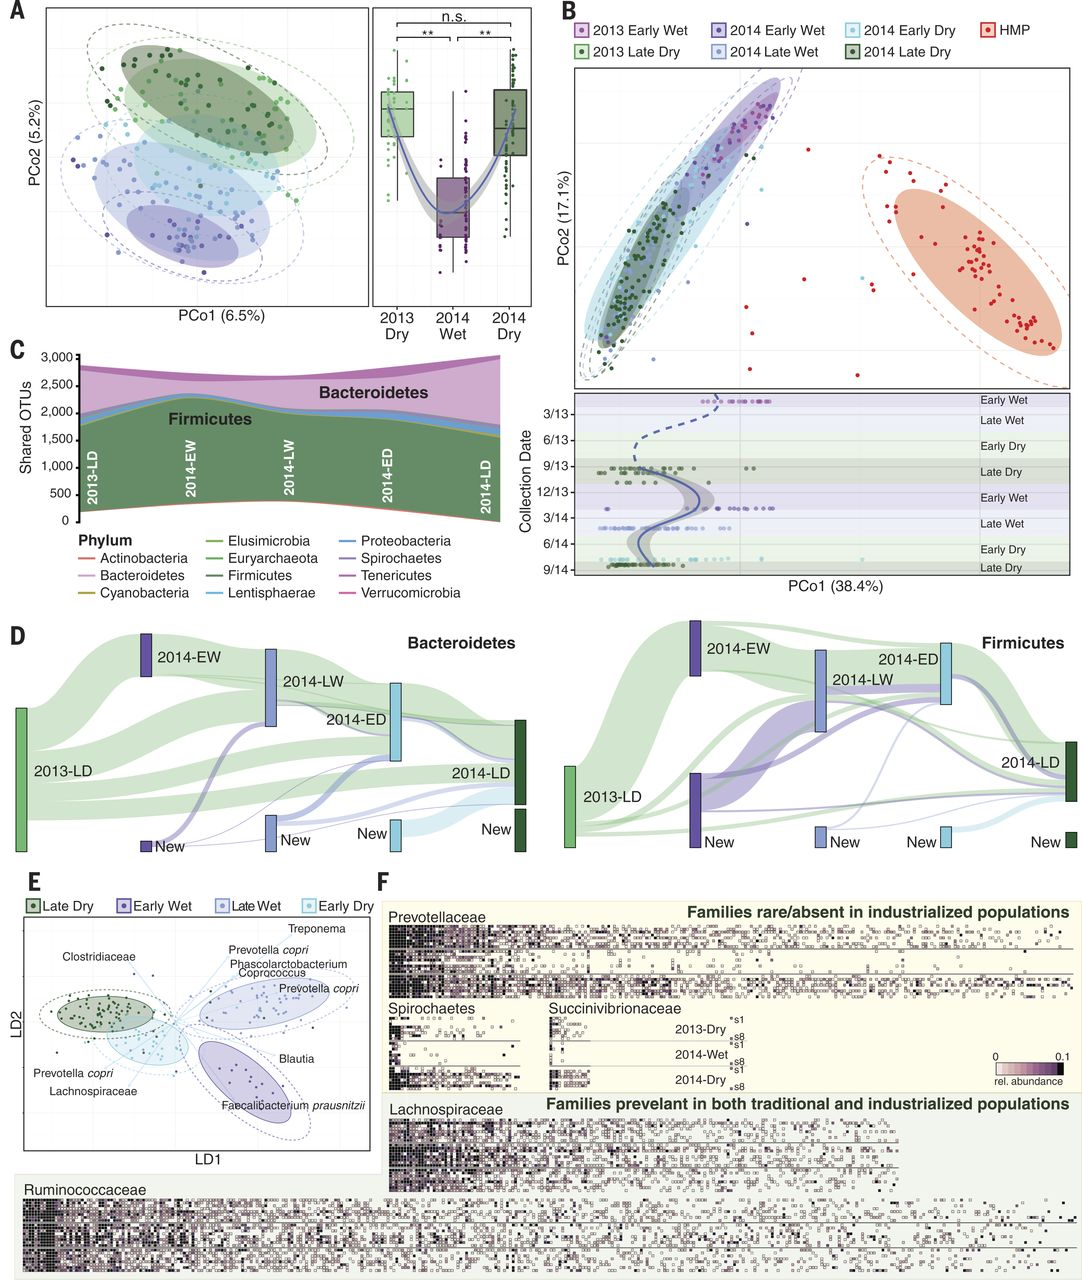
\includegraphics[width=1.0\paperwidth]{../figs/title_slide_example.jpg}}
\begin{frame}[plain] 

%  \vspace{15em}
\centering
%      \begin{figure}
      \begin{TitleBox}
   
      \vspace{.1cm} \centering \inserttitle
 
      \vspace{.5cm}

          {\normalsize January 21, 2020 \\ Caitlin Simopoulos }
       

      \vspace{0.5cm}

      {\normalsize  csimopou@uottawa.ca \\  \faGithubSquare~ \vspace{.5cm} \faTwitterSquare~ caitsimop} 
%    {\footnotesize \href{http://twitter.com/adaptive_plant}{{\FA \faTwitter} adaptive\_plant}
%    \href{http://www.falsters.net/daniel}{{\FA \faHome} www.falsters.net/daniel}
%    \href{mailto: daniel.falster@mq.edu.au}{{\FA \faEnvelope}  daniel.falster@mq.edu.au}
%    }
   \end{TitleBox}

  \end{frame}
    }
%~~~~~~~~~~~~~~~~~~~~~~~~~~~~~~~~~~~~~~~~~~~~~~~~~~~~~~~~~~~~~~~~~~~

\begin{frame}{Overview}
\be
\item What is reproducible data science?
\item Why is reproducibility essential when analyzing/visualizing data?
\item What is required to reproduce figures?
\item An example on how to be reproducible using R.
\ee

\end{frame}

%~~~~~~~~~~~~~~~~~~~~~~~~~~~~~~~~~~~~~~~~~~~~~~~~~~~~~~~~~~~~~~~~~~~
    \begin{frame} %{What is reproducibility?}
        \begin{block}{What is reproducible data science?}
           It is \textbf{raw data} and a set of instructions that explain \textbf{exactly} how you:
\bi
\item Completed your statistical analyses (from raw data)
\item Produced your figures and tables
 \ei
        \end{block}

    \end{frame}
%~~~~~~~~~~~~~~~~~~~~~~~~~~~~~~~~~~~~~~~~~~~~~~~~~~~~~~~~~~~~~~~~~~~

    
    \begin{frame}{Is this helpful?}

    \only<1>{\centering
    
\includegraphics[height=.8\textheight]{../figs/nature_2020.png}}

    \only<2>{
        \centering
    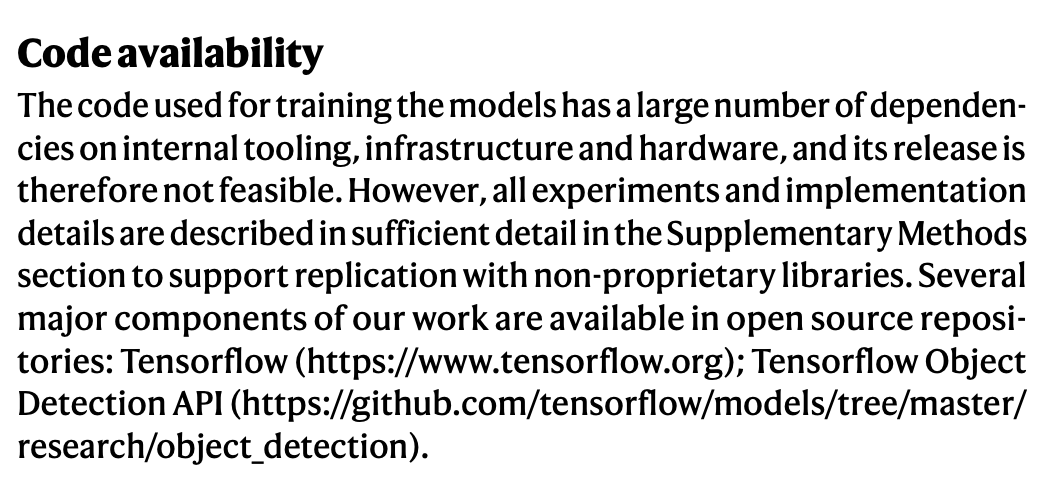
\includegraphics[height=.75\textheight]{../figs/code_avail.png}
    }

    \hfill\footnotesize Nature. 2020. https://doi.org/10.1038/s41586-019-1799-6
\end{frame}


%~~~~~~~~~~~~~~~~~~~~~~~~~~~~~~~~~~~~~~~~~~~~~~~~~~~~~~~~~~~~~~~~~~~
\begin{frame}{Why are we even talking about reproducibility?}

    \be
\item It saves \alert{you} time in the long run
    \bi
        \item Small OR big changes to figures are ``easy''
        \item Can create automated pipeline! ``Easy'' to do the same analysis on different data
    \ei
\item Journals often require code to be published so that the entire pipeline can be reproduced
    \bi
\item \alert{Shiny apps} ensure code will run and be used by researchers who may be uncomfortable with programming
    \ei
\item It's just good science
    \ee
\end{frame}
%~~~~~~~~~~~~~~~~~~~~~~~~~~~~~~~~~~~~~~~~~~~~~~~~~~~~~~~~~~~~~~~~~~~
\begin{frame}{What is required for reproducible analysis/figs?} 

    \be
\item Raw data
\item Code used to \alert{normalize} and \alert{analyze} data 
\item Output data file that can be directly visualized (\alert{optional})
\item File that discloses software/package versions; download date of any files used (\textit{e.g.} databases)
\item A ``README'' file that explains how to use your code 
    \bi
\item can include previous point
    \ei
\item An \alert{organized} repository to store these required files 
    \ee 
    \only<2>{ \centering\alert{Everything needed to get someone from raw data to your figures.}}
\end{frame}
%~~~~~~~~~~~~~~~~~~~~~~~~~~~~~~~~~~~~~~~~~~~~~~~~~~~~~~~~~~~~~~~~~~~
\begin{frame}{An example:}

    \centering
    \Large\url{https://github.com/caitsimop/reproducible-figs}

\end{frame}    
%~~~~~~~~~~~~~~~~~~~~~~~~~~~~~~~~~~~~~~~~~~~~~~~~~~~~~~~~~~~~~~~~~~~
\begin{frame}{Notice the directory/folder structure}
    \begin{columns}
        \column{.4\textwidth}

\centering
        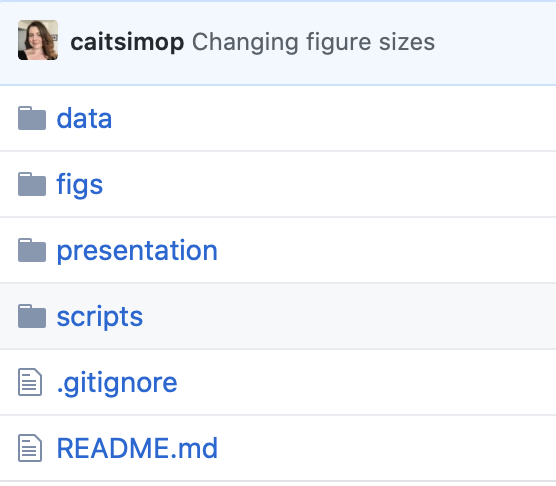
\includegraphics[width=\textwidth]{../figs/directory.png}
        \column{.6\textwidth}
        \bi
    \item Organized 
    \item Obvious
    \item Includes ALL files needed
\ei
    \end{columns}
\end{frame}
%~~~~~~~~~~~~~~~~~~~~~~~~~~~~~~~~~~~~~~~~~~~~~~~~~~~~~~~~~~~~~~~~~~~
\begin{frame}%{What to include in the README}

\centering
\large
    Follow along with me in R (if you want), or just watch me on the screen 

\end{frame}    
%~~~~~~~~~~~~~~~~~~~~~~~~~~~~~~~~~~~~~~~~~~~~~~~~~~~~~~~~~~~~~~~~~~~
\end{document}
